\documentclass[12pt]{article}
\usepackage{amssymb,latexsym,fullpage,epsfig}



\newcommand{\buttonFig}[1]{
\parbox[c]{1em}{\vspace{0em} \includegraphics[width=1em]{#1} }
} 

\begin{document}


\title{Sleep Is Death (Geisterfahrer)}

\date{}

\maketitle
%\thispagestyle{empty}


\vspace{-0.9in}

\begin{center}
{\Large \it Controller Interface Guide}
\end{center}


%\section{Overview}
{\it Sleep Is Death} is a two-player, turn-based game.  One person plays as the ``Player,'' and the other plays as the ``Controller.''

The Player commands the behavior of a single character in the world.  Hopefully, the world and other objects react coherently to the Player's actions---it is the Controller's job to ensure this coherence.  The Controller commands the behavior of all the other characters and objects in the world, essentially fabricating an interactive illusion that folds around the Player.

%The user interface shown to the Player is too simple to warrent explanation.  The Controller's interface, on the other hand, is quite complex.  However, the Controller's interface was designed to be as simple as possible while still allowing the Controller to {\it quickly} manipulate every aspect of the game world.  

The Controller's interface is comprehensive.  Swapping rooms, swapping objects, editing speech, moving things around, and editing the soundtrack are all at your fingertips.  Deeper levels of the interface also support editing rooms and objects on the fly, a technique that becomes necessary for advanced Controller play.

The basic Controller interface is show below:
\begin{center}
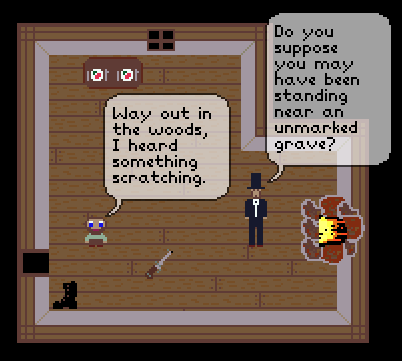
\includegraphics[width=0.6\textwidth]{screen.eps}
\end{center}
If your screen doesn't look like this, you may be down inside one of the sub-editors.  Look for a Close button (\buttonFig{close.eps}) in the upper-left corner of the screen.  Press Close until you back out to the basic screen shown above.  If you want to return to a ``clean slate'' at any point, press the Clear button:
\begin{center}

\includegraphics[width=3em]{clear.eps}
\end{center}
Tool tips are provided for every button in the game.  Some of the more subtle aspects of Controller play are described on the following page.


\paragraph{Turn structure}  Each side has {\it 30 seconds} to commit a move, one after the other.  The timer for your move is shown in the upper left corner of the screen.  When the counter reaches 0, your move is sent.  Your counter goes negative during the other player's move, but jumps back up to positive 30 again when it's your turn.

During the Controller's move time, the Player's view is frozen in a ``Waiting...'' state.  The Controller manipulates the state of the world, and after the Controller's move is sent, the Player's view is updated to match that state.  During the Player's move time, the Controller can continue to manipulate the world, behind the scenes, in anticipation of the move that the Player will eventually send.  These behind-the-scenes manipulations are invisible to the Player.  %Thus, while the Player has only 30 seconds to pick a move, the Controller effectively has 60 seconds.  This extra time can be used to prepare new objects and rooms for potential future needs in the game.

\paragraph{Game resources}  Objects and Rooms in the game can be browsed and selected with the Picker interfaces on the right side of the screen.  These interfaces can be toggled between Stack and Search modes with the \buttonFig{stack.eps} and \buttonFig{search.eps} buttons.  The game state's Room will switch to whatever Room is selected in the picker.  Objects are a bit different, though, as picking an Object doesn't automatically alter the game state.  Instead, pressing this button will replace the current Object in the game state with the selected Object from the Picker:
\begin{center}

\includegraphics[width=3em]{replace.eps}
\end{center}

\paragraph{Manipulating Objects}  The toolbar at the bottom of the screen allows you to manipulate Objects in the game state in various ways.  Undo and Redo buttons are also provided, so there's no danger in making a mistake.

\paragraph{Going deeper} Every resource in the game is fully editable, should the need arise.  Look for the Edit buttons (\buttonFig{edit.eps}) at the top of each picker to enter a sub-editor.  Some of these have further sub-editors.  Whenever you edit a resource, your new version of that resource is added to the database.  You can then use your new version in the current game state by backing out to the main state editor (press the Close button, \buttonFig{close.eps}, in the upper left corner).



\end{document}
